%%%%%%%%%%%%%%%%%%%%%%%%%%%%%%%%%%%%%%%%%%%%%%%%%%%%%%%%%%%%%%%%%%%%%%%%%%%%%%%%
% experiment.tex: Chapter describing the experiment
%%%%%%%%%%%%%%%%%%%%%%%%%%%%%%%%%%%%%%%%%%%%%%%%%%%%%%%%%%%%%%%%%%%%%%%%%%%%%%%%
\chapter{The CMS Experiment}
\label{experiment_chapter}
This chapter details the CMS experiment as well as the CERN accelerator, the Large Hadron Collider (LHC), which is used by CMS. Specific attention is paid to the components of CMS and the LHC most relevant to the \WR search.
The \LHC is the largest and highest energy particle collider ever created.  It is a 27 kilometer circumference synchrotron accelerator.  With two beam pipes each designed to carry approximately 2700 bunches of protons which can be brought into collision at four interaction points around the ring.  The four experiments around the ring clockwise looking down are \ALICE, \CMS, \LHCb, and \ATLAS.  It was first operated with \rootsseven, then \rootseight, and now \rootsthirteen.

\begin{figure}[!htbp]
    \centering
    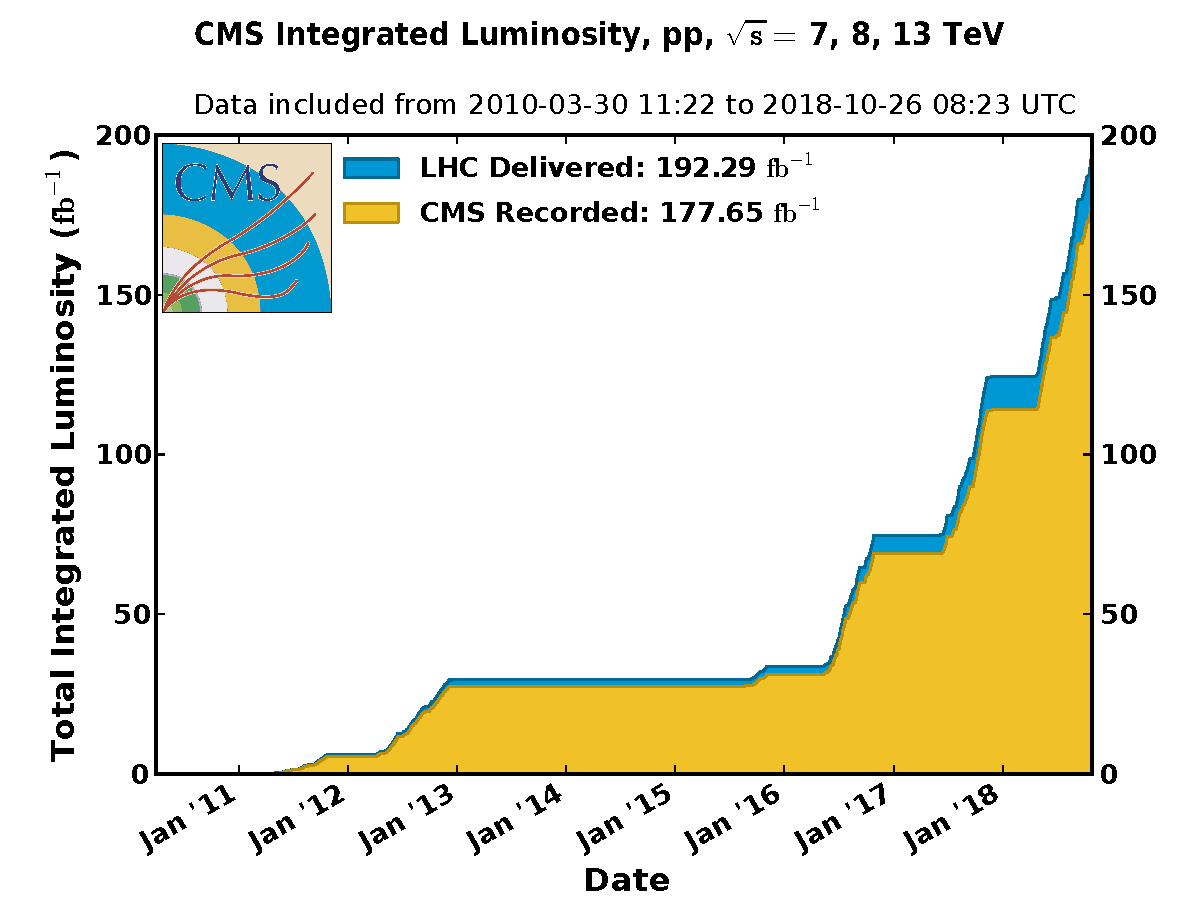
\includegraphics[width=\textwidth]{figures/int_lumi_allcumulative_pp.pdf}
    \caption[
        %short caption
        Multi-year delivered luminosity of the \LHC
    ]    
    {
        This graph shows the integrated luminosity of the \LHC over all the years of operation.  It can be seen that recent years have seen a dramatic increase in instantaneous luminosity, with the last year, 2018, contributing approximately one third of the total.
    }
    \label{fig:lhc_delv_lumi}

\end{figure}

\section{The Large Hadron Collider}
The \LHC was constructed in Meyrin, outside Geneva, Switzerland.  It was first operated in the Fall of 2008, and after a magnetic failure, was repaired and recommenced operation in 2010.  2010 saw \GLNTEN delivered luminosity at \rootsseven.  The accelerator continued at this energy for 2011 delivering \GLNELEVEN.  In 2012 the energy increased to \rootseight and delivered \GLNTWELVE.  After a longer shutdown for three years and significant upgrade work, the \LHC resumed operation at \rootsthirteen and ran for 2015, 2016, 2017, 2018.  \GLNTOTALII was delivered over those four years.

The \LHC accelerator is part of an accelerator system, starting at low energies and progressively increasing the energy.  The start of the \LHC proton beam is a humble gas bottle of hydrogen gas.  From there, the gas is ionized and accelerated with a linear accelerator LINAC 2.  LINAC 2 accelerates protons directly into the Proton Synchrotron (PS).  The PS accelerates the protons to an energy of \SI{26}{GeV}.  Protons from the PS are then injected into the Super Proton Synchrotron (SPS).  The SPS accelerates proton bunches up to \SI{450}{GeV}.  Once proton bunches have reached this energy they can be accelerated into the \LHC. These bunches are then accelerated to 6500 \GeV.  The \LHC was originally designed for operation at up to \rootsfourteen but has not done so yet, in the last data taking period, which concerns this analysis, the \LHC ran at \rootsthirteen.

Protons are accelerated in each of the synchrotons with radio-frequency (RF) cavities.  The RF cavities fill a cavities in the beam path with standing electro-magnetic waves in the radio frequency range.  Protons passing through the standing waves are accelerated and kept in bunches.  Slow (and behind) protons are accelerated more than faster (and leading) protons in each bunch. This ensures that each bunch of protons is well formed in momentum and physical space.  At the LHC there a 8 RF cavities for each beam and are operated at \SI{400}{MHz}.  Bunches collide at intervals of \SI{25}{ns}.  This is part of the design of the RF cavities, as the each bunch is accelerate every 10 cycles of the radio frequency.  This gives a maximum number of bunches at the LHC of roughly 3600.  Each step in the synchrotron acceleration chain requires additional space so that injection (and dumping) magnets can be brought to full energy in between bunches.  This gives an actual total of 2808 bunches.

While the \LHC has held the record for the highest center of mass energy per nucleon of any hadron collider built to date, which allows it to probe previously unreached mass regions, it is also the most luminous hadron collider.  The record instantaneous luminosity and a high-duty cycle has allowed the \CMS experiment to record an unprecedented number of collisions.  The luminosity is proportional to a number of factors

\begin{equation}
    \luminosity = \frac{fnN^{2}\gamma}{4\pi\epsilon_{n}\betastar}F
    \label{eq:lumieq}
\end{equation}

\ensuremath{f} is the frequency a given bunch interacts, \ensuremath{n} is the number of bunches protons in each beam, \ensuremath{N} is the number of protons in each bunch, \ensuremath{\gamma} is the Lorentz boost of the protons, \ensuremath{\epsilon_{n}} is the beam emittance, \betastar is the beta function, and \ensuremath{F} is based on the shape of the beam crossing.  Emittance and the beta function describe the focusing of the beams as they cross.  Multiplying them together gives the square of the cross-section area of the beams at the crossing point.  At the \LHC the number of protons per bunch, the number of bunches and the beam cross-section at collision can be changed.  It can be seen from \ref{eq:lumieq} how these parameters affect the luminosity.  Increasing the number of bunches and the protons per bunch increase luminosity.  Likewise, focusing the beams to a small cross-section increases luminosity.  Each of these variables have their limits and challenges associated with changing them.  The total number of bunches the \LHC can hold is predefined by the frequency of the RF cavities as well as the need for injection and ejection of the beams in the accelerator chain.  The number of protons per bunch, while keeping a bunch size the same, or conversely keeping the number of protons per bunch the same and reducing bunch size can be done but is technically difficult.  Higher proton density bunches are more difficult to control and can become unstable.  Higher proton density in bunches also leads to an increase in additional proton interactions in a given crossing.  This poses a challenge to the detectors to sufficiently determine the properties of the interaction of interest and increases the rate of radiation damage in the detector. During Run II, 2015-2018, the \LHC was operated at its tightest bunch spacing of \SI{25}{ns}.  2015 was considered a commissioning year and collected significantly less data and is not considered in this analysis.  From 2016-2018 the \LHC continued to outperform itself, increasing the number of protons per bunch beyond design specifications and ultimately delivering \GLNTOTALII collisions.  Some of the relevant parameters for the three years covered in this analysis are shown in \ref{tab:lhc_design_specs}.

\begin{table}[]
    \centering
    \begin{tabular}{|c|c|c|c|}
        \hline
        Parameters & 2016 & 2017 & 2018\\
        \hline
        Beam Energy & \SI{6.5}{TeV} & \SI{6.5}{TeV} & \SI{6.5}{TeV}\\
%        \betastar & \SI{IDK}{m} & \SI{IDK}{m} & \SI{30}{cm}\\
        Bunch Spacing & \SI{25}{ns}& \SI{25}{ns}& \SI{25}{ns}\\
        Number of Bunches & 2808 & 2808 & 2808 \\
 %       Protons per Bunch & & & \\
  %      Normalized Emittance at Start of Fill & & & \\
        Peak Luminosity Per Day & \SI{15.3}{Hz/nb}& \SI{20.7}{Hz/nb}& \SI{21.4}{Hz/nb}\\
        Mean Number of Events per Crossing & 27& 38& 37\\
        Delivered Integrated Luminosity & \GLNSIXTEEN& \GLNSEVENTEEN& \GLNEIGHTEEN\\
        \hline
    \end{tabular}
    \caption[LHC operating parameters]{Operation parameters of the LHC during Run II, 2016-2018.}
    \label{tab:lhc_design_specs}
\end{table}

\begin{figure}[!htbp]
    \centering
    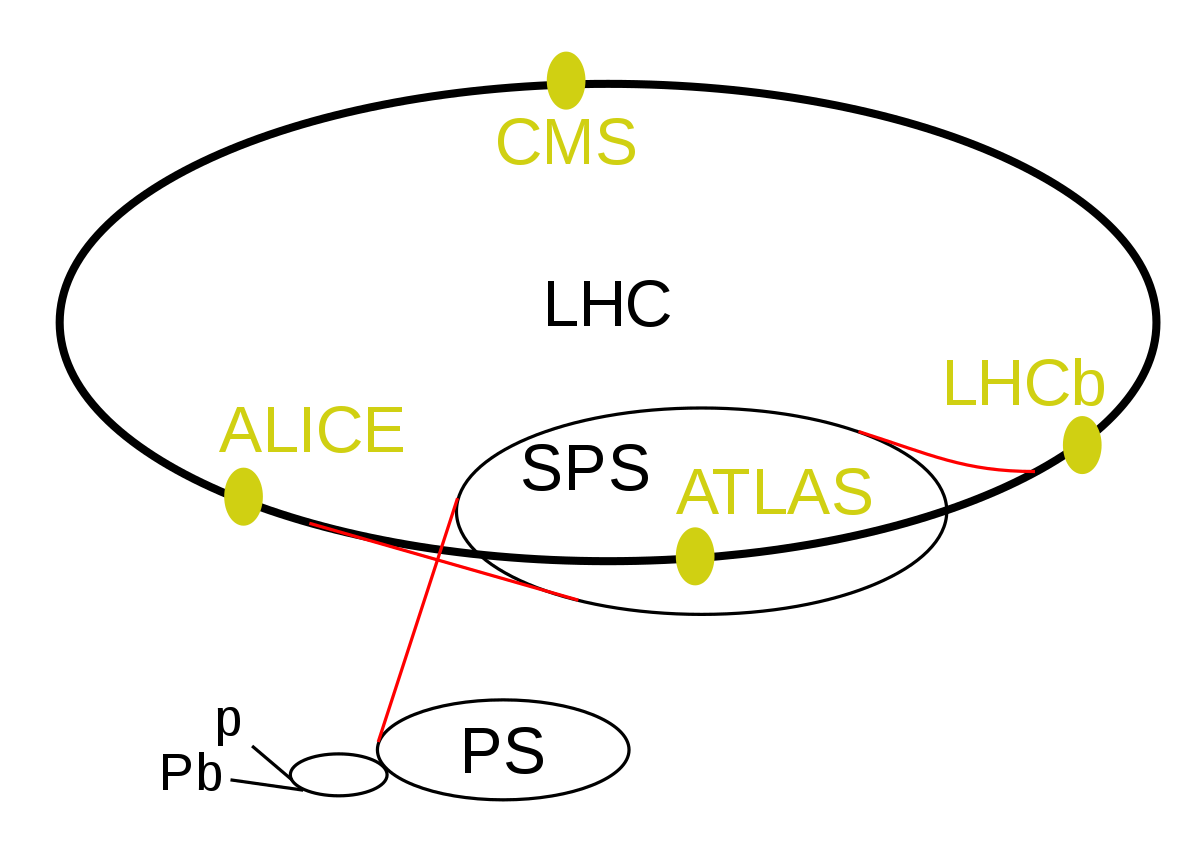
\includegraphics[width=\textwidth]{figures/1200px-LHC_svg.png}
    \caption[
        %Short caption for the list of figures
       LHC accelerator complex.
    ]{
        % Full caption shown below the image
        This diagram shows the accelerator complex feeding into the LHC.  Starting with a linear accelerator, the protons are accelerated into the Proton Synchrotron (PS) and then Super Proton Synchrotron (SPS) before injecting into the LHC. 
    }
    % A label so you can \ref{fig:my_fig}. It is arbitrary; neither the 'fig:'
    % nor the fact that it has the same name as the pdf are required.
    \label{fig:lhc_diag}
\end{figure}



\section{The Compact Muon Solenoid}
The Compact Muon Solenoid (\CMS) at CERN is one of the general purpose detectors at the \LHC and the one used for this analysis.  Each part of the detector is built around the next moving outward from the interaction point in a cylindrical shape.  Through the long axis of \CMS runs a single beam-pipe containing both proton beams which are brought into collision in the very center. \CMS is designed to accept as many events as possible and with as much detail as possible.  It covers a large solid angle to allow for as many of the post-collision particles to encounter an active part of the detector.  \CMS also has extremely fast electronic readout to allow it record events as often as possible and as accurately as possible.  \CMS is divided into several layers each with overlapping components to allow for as much acceptance as possible.

The CMS detector has several major detector components, sub-detectors, as well as a very large solenoid magnet.  The support for these components is integrated as part of the magnet return yoke.  Starting at the interaction point and moving outward transversely, the CMS detector is made up of a silicon-tracker, an electromagnetic calorimeter (ECAL), a hadronic calorimater (HCAL), the magnet, and then the muon chambers with an iron magnet return yoke interspersed.  Each of these parts will be discussed further shortly.

Additionally the detector changes on the two ends of the cylinder, called endcaps, this is to account for the differing particle fluence at different collision angles.  A drawing a \CMS and it's different components is shown in \cite{Sakuma_2014}.

As the \CMS detector is discussed it's first helpful to describe the coordinate system used.  This coordinate system is standard for hadron collider experiments.  The Cartesian coordinates are defined as follows: \ensuremath{x} points to the center of the collider, the \ensuremath{y} points up, and the \ensuremath{z} coordinate points in the counter-clockwise, looking down, direction along the beam.  This creates a right-handed coordinate system.  The origin of these coordinates lies at the center of collisions within the detector.  Another coordinate system is also defined to better reflect the geometry of the particle collisions and the detector itself.  This coordinate system is defined with \ensuremath{\eta}, \ensuremath{\phi}.  \ensuremath{\phi} is simply the azimuthal angle in the \ensuremath{x-y} plane.  \ensuremath{\eta} is defined as pseudo-rapidity.

\begin{equation}
    \eta \equiv - \ln{
    \tan \left(\frac{\theta}{2}\right) }
    \label{eq:pseudorapidity}
\end{equation}

Here \ensuremath{\theta} is the the polar angle along the \ensuremath{z} axis.

Pseudo-rapidity is used as a simpler alternative to particle rapidity defined with the particle momentum along the beam direction and it's energy.

\begin{equation}
    Y \equiv \frac{1}{2} \ln{\left( \frac{E+p_z}{E-p_z} \right)}
    \label{eq:rapidity}
\end{equation}

When a particle is massless, the \ensuremath{Y} simplifies to \ensuremath{\eta}, which is a good approximation considering the energies of particles at the \LHC.
At \LHC energies proton collisions actually involve the collision of individual components of the protons, quarks and gluons.  The momentum of these partons is not known during the collision.  The result is that each collision has a different amount of boost along the \ensuremath{z} axis.  
However, the rapidity of a particle does not change when the particle is boosted.  As such, defining a coordinate system with \ensuremath{\eta} which approximates \ensuremath{Y} allows for post-collision particle directions to be discussed in a way roughly invariant of their initial momentum in the \ensuremath{z} direction.  Given the large inelastic cross-section at the \LHC, this also guarantees that any given sweep of \ensuremath{\Delta \eta} will have roughly the same particle fluence.

As a result of the unknown longitudinal momentum, particle's momentum and energy is generally only considered in the transverse direction.  The transverse components are calculated from \ensuremath{\eta}.  The transverse momentum and energy of a particle is defined as
\begin{equation}
    p_T \equiv |p| / \cosh{\eta} 
    \label{eq:pT}
\end{equation}{}
\begin{equation}
    E_T \equiv E / \cosh{\eta} 
    \label{eq:Et}
\end{equation}{}

Energies and momentums determined from the detector can then be re-expressed independent of the particle's longitudinal boost.  \ensuremath{\eta} and \ensuremath{\phi} are also used in conjunction to calculate particle's separation independent of their longitudinal momentum as well.  This is defined as \ensuremath{\Delta R}
\begin{equation}
    \Delta R \equiv \sqrt{\Delta\eta^2 + \Delta\phi^2} 
    \label{eq:dR}
\end{equation}{}
\subsection{Tracker}
The tracker is the at the center of \CMS.  It provides the basis of the reconstruction of particles passing through the detector from the collision point.  All particles travelling into \CMS with a \ensuremath{|\eta| < 2.5} from the interaction point pass through the tracker.  Their are two main parts of the tracker: the strip tracker and the pixel detector, each made with silicon.  The strip tracker is used primarily for measuring momentum, and the pixel detector for position.
Silicon detectors operate by collecting ionized charge in material.  Each active region in the detector gives an interaction location for the particle, and an amount of charge ionized in the material, which is a function of the particle's momentum and charge.  Silicon was chosen to satisfy the stringent requirements of the detector, that it have a very refresh time (faster than the time between interactions of \ensuremath{\SI{25}{ns}} and be radiation hard.  As the tracker is closest to the beam line of all sub-detectors, the tracker must have high-resolution.

The tracker is, at it's closest, just \ensuremath{\SI{4.4}{cm}} from the interaction point.  The region closest to the interaction point is cylindrical and made up of several layers, each \ensuremath{\SI{53}{cm}} long.  At higher \ensuremath{\eta} the orientation of the detector changes and is made up of several layers of discs.

Each pixel in the tracker is just \ensuremath{100\times150 \mu m}.  Individual particle crossing positions are determined with weighted averages based on the amount of charge left in each pixel, which also for determining of the position beyond the pixel scale.  Charged particles additionally bend in the magnetic field of \CMS angling their interaction with tracker, leading to more spread.

The strip tracker sits around and outside the pixel tracker.  The strip tracker allows for momentum determination of charged particles, by measuring the track curvature.  With the high magnetic field of \CMS and a longer distance from the interaction point, the measurement is improved over just the pixel detector.  While a pixel detector could be built in the place of the strip tracker, this is not practical.  Each strip runs the length of a tracker module and is between 80 and 180 \ensuremath{\mu m} wide depending on it's distance from the interaction.  While these are clearly much larger than the pixel detector's pixels, each track's curvature based on the magnetic field lies in a plane transverse to the beam-line.  A cross-sectional view of the strip tracker can be seen in \ref{fig:tracker}.

\begin{figure}[!htbp]
    \centering
    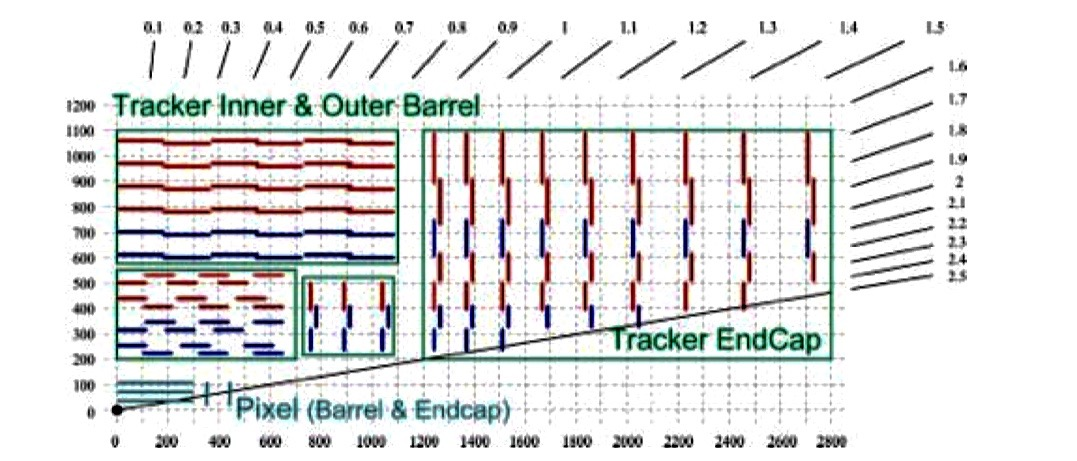
\includegraphics[width=\textwidth]{figures/Tracker.jpeg}
    \caption[
        %Short caption for the list of figures
       \CMS tracker diagram.
    ]{
        % Full caption shown below the image
        A cross-section of a part of the \CMS tracker is shown.  The \ensuremath{\eta} is shown on the around the top-right.  The distance from the interaction point is on the bottom-left in millimeters.  Blue and Red modules are shown, the red being one sided and the blue two sided. \cite{trackerPerf}
    }
    % A label so you can \ref{fig:my_fig}. It is arbitrary; neither the 'fig:'
    % nor the fact that it has the same name as the pdf are required.
    \label{fig:tracker}
\end{figure}

One of the most significant challenges in using the tracker to it's full potential is alignment.  The position of the tracker's components and the position of the tracker relative to the rest of \CMS has to be known to better than the tracker's own resolution.  This alignment calibration has to be done completely in-situ and repeated at regular intervals.  Cosmic-ray muons serve this purpose very well.  Both with and without the magnetic field of \CMS turned on, the passage of these muons through the detector (and out the other side) allow for this alignment.  Performance of the tracker is further understood using very well known standard model processes common in the proton-proton collisions at the \LHC.  The \Ztomumu process is studied for this.  The shape of the reconstructed mass of the \Z as a function of one of the muon's angle \ensuremath{\phi} reveals possible distortions in the tracker which can be corrected.

The precision of the tracker is ultimately key for identify the primary interaction vertex in the event, this allows for the rejection of particles stemming from an uninteresting vertex (pileup).  In the transverse plane it's resolution is on the order of \ensuremath{\SI{100}{\mu m}} and longitudinally, \ensuremath{\SI{150}{\mu m}}.  The resolution of a muon with \ensuremath{\SI{100}{\GeV}} is approximately \ensuremath{1\%} in the barrel region and \ensuremath{3-6\%} in the endcap region.  For more information about the tracker see \cite{trackerPerf}.

\subsection{Electromagnetic Calorimeter}
The electromagnetic calorimeter (\ECAL) absorbs and measures the energy of charged particles passing through it.  Electrons and photons are typically completely stopped in the \ECAL, while quark-matter particles will leave some energy and continue through to \HCAL.  \ECAL is a total absorption calorimeter with an active material made out lead-tungstate crystal.  Each crystal absorbs the energy of particles moving through by electromagnetic interactions, this energy is then converted to scintillation light.  The magnitude of this light is then measured.

\begin{figure}[!htbp]
    \centering
    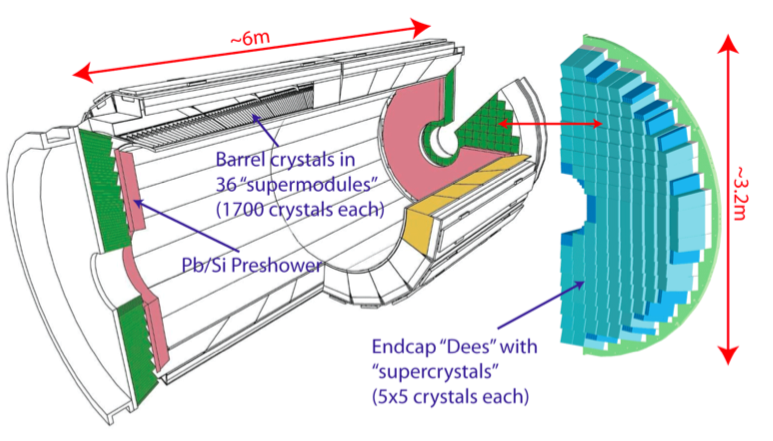
\includegraphics[width=\textwidth]{figures/ECAL_diag.png}
    \caption[
        %Short caption for the list of figures
       \CMS \ECAL diagram.
    ]{
        % Full caption shown below the image
        This cut-away of the \ECAL shows the barrel and endcap regions, as well as the pre-shower.  Individual crystals and their alignment towards the nominal interaction point can be seen. \cite{ecalPerf}
    }
    % A label so you can \ref{fig:my_fig}. It is arbitrary; neither the 'fig:'
    % nor the fact that it has the same name as the pdf are required.
    \label{fig:ecal}
\end{figure}

\ECAL is divided into three sections covering all of \ensuremath{\phi} and out to an \ensuremath{\eta} of 3.0.  There are the barrel, end-cap and pre-shower sections.  The barrel and end-cap have the same design, but with a different orientation of the detector, though the crystals all still point to the interaction point at the center of \CMS.  As \ECAL is designed to surround the tracker, all of the power, readout, and cooling pipes for the tracker must pass through \ECAL somewhere.  There is a gap between the barrel and endcap sections of \ECAL to allow for this.  This gap is angled such that a very minimal amount of area goes undetected.

Each crystal of lead-tungstate in \ECAL in the barrel region is \ensuremath{2.2\times \SI{2.2}{cm^2}} and \ensuremath{\SI{23}{cm}} long.  In the endcap they are slightly wider and shorter at \ensuremath{2.86\times \SI{2.86}{cm^2}} and \ensuremath{\SI{22}{cm}} long.  These crystals are arranged in \fivebyfive groups arranged to be rectangular in \etaphi.  The long axis of the crystals are not perfectly aligned, and are \ensuremath{\SI{5}{\deg}} off.  This reduces the chance that a particle travelling from the interaction point proceeds along the gap between crystals. \ensuremath{\SI{6}{m}} long.  The \ECAL has a total of 61200 crystals in the barrel and 7324 crystals in the endcap.

In additional to the crystals used in \ECAL, covering most of the endcap section is a part of the detector called the pre-shower.  The pre-shower is a silicon detector which has much higher resolution than the endcap section of \ECAL.  The high spatial resolution was intended to improve the ability to determine the difference between single photons and boosted \pitogammagamma decays.  However, it was not effective for this.

\ECAL is the first usage of lead-tungstate, \leadtungstate, in a calorimeter.  Lead-tungstate (as crystallized for \CMS) is clear, and it's high density gives it a radiation length of just \ensuremath{X_0 = \SI{0.89}{cm}} and a Moliere radius of \ensuremath{\SI{2.2}{cm}}.  Radiation lengths are a way of standardizing the amount of absorption that will occur in the detector.  The Moliere radius has to do with the volume over which the shower of energy spreads.  The short radiation length of the crystal allows \ECAL to be smaller, and the small Moliere radius allows for higher spatial resolution in the detector.

The disadvantage of lead-tungstate is it's low light yield.  With only \ensuremath{ \SI{30}{photons/\MeV}}, approximately.  High-gain photo-sensors are used to amplify this signal.  The barrel region uses avalanche photo-diodes (APDs) and the endcaps use vacuum photo-triodes (VPTs).  Each has a high gain, while remaining relatively insensitive to the high magnetic field environment they operate in.  Signals coming from each crystal are digitized and stored in electronics on the detector, the front-end, and are only readout on request by the \CMS trigger system.  This reduces the data rate for \ECAL, as sending all of the information for all crystals each collision would not be feasible.

The best performance of \ECAL requires near-constant calibration.  As with all detector components of \CMS, lead-tungstate is radiation hard.  However, the crystal structure is slowly damaged by radiation, as imperfections in the crystal, reducing the light produced from an interaction.  To maintain the highest possible precision, \ECAL is regularly recalibrated with a built-in laser system, which can operate during the abort-gap of the \LHC while physics data is taking in collisions.

\ECAL was first calibrated with dedicated beams and radioactive sources prior to being installed in \CMS.  With a known source, the whole detector can be calibrated such that there is no asymmetry in the response based on \etaphi.  The absolute calibration of the detector is also done with physics collisions in \CMS using the \Z boson.  It's mass is very well understood from independent measurements and the signal is visible strongly over background.  The resolution is function of energy and is parameterized as:

\begin{equation}\label{eq:ecal}
    \frac{\sigma_{E}}{E}
    =   
    \frac{\SI{2.8}{\%}}{\sqrt{E/\left(\SI{1}{\GeV}\right)}}
    \oplus
    \frac{\SI{0.128}{\GeV}}{E}
    \oplus
    \SI{0.3}{\%}.
\end{equation}

More details on the performance of \ECAL can be found in \cite{ecalPerf}.

\subsection{Hadron Calorimeter}
The hadron calorimeter (HCAL) sits outside the ECAL and samples the energy from hadrons produced in collisions.  The HCAL also stops most of the remaining particles, muons and neutrinos being the most common exception.

There are four sub detectors in HCAL: HB, HE, HF, HO.  These correspond to the barrel, endcap, forward and outer regions.  HB, HE and HO follow the same overall design.  Each is made out of layers of brass and plastic scintillator.  The brass is used to absorb the energy of hadrons passing through and cause them to shower. The energy of these showers is then measured in the subsequent plastic scintillator layer. Showers often pass through several HCAL layers before being totally absorbed.  The energy in each of these depths can then be summed for a total energy measurement, or compared to give more information on the shower evolution. A cross-section of HCAL with the regions HB, HE, and HO cover is shown in figure \ref{fig:hcal}.

\begin{figure}[!htbp]
    \centering
    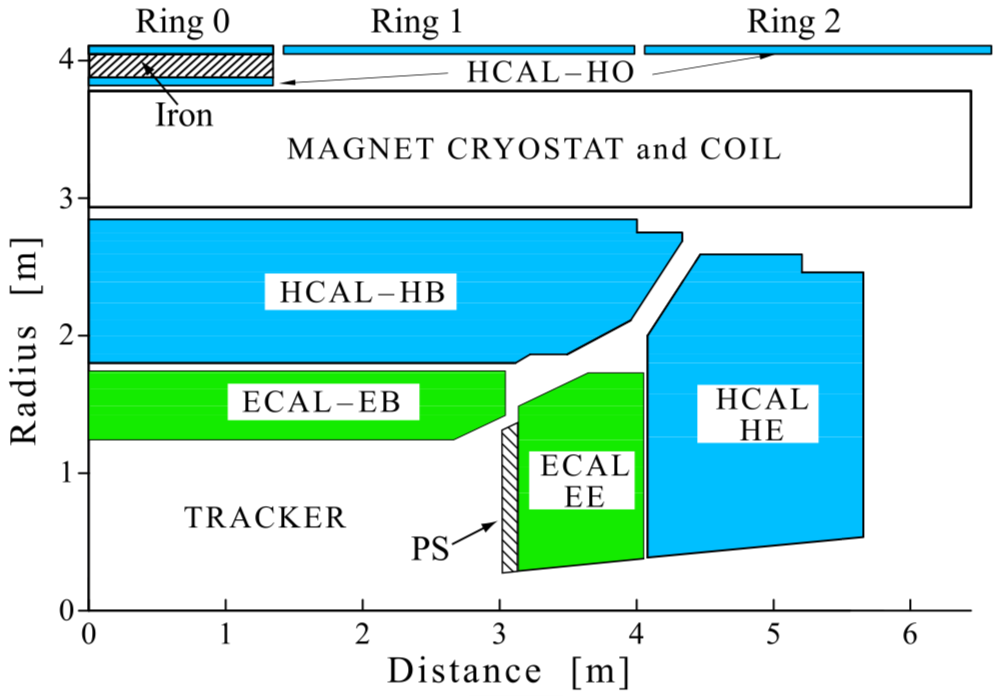
\includegraphics[width=\textwidth]{figures/HCAL.png}
    \caption[
        %Short caption for the list of figures
       \CMS \HCAL diagram.
    ]{
        % Full caption shown below the image
        This cut-away of the \HCAL shows the barrel and endcap regions, and it's arrangement with adjacent \CMS components.  The barrel and endcap regions are within the magnet. The gap between them allows for cabling to the inner detector. HF is not pictured as it sits separately in a higher \ensuremath{\eta}. \cite{HCALperf}
    }
    % A label so you can \ref{fig:my_fig}. It is arbitrary; neither the 'fig:'
    % nor the fact that it has the same name as the pdf are required.
    \label{fig:hcal}
\end{figure}

HF is the most forward part HCAL and the most forward detector used in event reconstruction.  It covers the \ensuremath{|\eta|} of up to 5.0.  As a result of the significantly higher particle flux in the forward regions, HF has a special, exceptionally radiation hard design. The bulk of HF is comprised of steel, with quartz fibers running horizontally through it.  These quartz fibers measure the energy of particles passing through them by the direct Cerenkov radiation produced in them. Each channel in HF comprises two such fibers, one short and one long. The long fibers run the length of HF, whereas the short end farther from the inward side.  The difference between the energy deposited in the fibers can be used to determine how deeply the transiting particle showered, which is related to whether the particle is a photon or lepton as opposed to a hadron, which will shower deeper in.

\HCAL has been specifically designed to measure the energy of hadrons.  Hadrons, being composite particles of quarks, have a complicated shower structure.  They are also generally more penetrating than electrons or photons, which are effectively absorbed in \ECAL.  Quarks and gluons cannot travel through space freely, as they carry color.  Only color neutral combinations travel, and these are most commonly pions.  Pions are light quark anti-quark pairs.  Neutral pions decay quickly and to leptons, which is well absorbed in \ECAL.  Charged pions, however, decay more slowly, via the weak-force.  These, as well as neutrons and protons from the collision, pass through \ECAL.  Any electrically charged hadron will interact with the tracker and \ECAL, leaving some energy.  As they are much heavier than electrons, they are not stopped as easily through electromagnetic interactions.  Hadrons will, however, interact with the strong force on nuclei in the detector.  This happens in \ECAL as well as \HCAL.  Each interaction can create more hadrons with energy sufficient to continue travelling through the detector.  The energy of the initial hadron is then distributed throughout \ECAL and \HCAL and requires a more careful reconstruction.

The specific ratio of neutral and charged pions involved in a shower is inherently random.  Each shower will contain different amounts.  Since each shower is started by only tens of hadrons, these fluctuations can be significant.  The calorimeters do not have the same response to the electromagnetic interactions from neutral pion decays and the nuclear interactions of charged pions.  This results in a degraded resolution of \HCAL from what might be theoretically expected.  The behavior of the detector response with respect to different hadrons, and the distributions of them in a shower have to be understood to make accurate measurements.

The \CMS \HCAL has 17 plastic scintillator layers each \ensuremath{\SI{3.7}{mm}} thick with the first and last layers thicker at \ensuremath{\SI{9}{mm}}.  In between each of the middle layers is brass absorber.  The outer layer being stainless steel.  The first layer is \ensuremath{\SI{61}{mm}} thick.  The eight layers after are thinner at \ensuremath{\SI{50.5}{mm}}.  The next six are slightly thicker at \ensuremath{\SI{56.5}{mm}}.  The last layer is the \ensuremath{\SI{75}{mm}}.  The initial layer's extra thickness helps catch showers which might begin in the gap between \ECAL and \HCAL, these would be impossible to reconstruct well.  The last layer is the thickest to attempt to stop any shower from continuing past \HCAL, though a few still will.  Outside of the \CMS magnet is another small layer, HO, meant to catch the most penetrating of showers.  Combining \ECAL and \HCAL, there are between 7 and 10 interaction lengths depending on the part of the detector.

Signal amplification from the plastic scintillators was originally done with hybrid photo-diodes.  These are in the process of being replaced, however, with silicon photo-multipliers (SiPMs).  SiPMs offer improved resolution improving detector performance despite radiation degradation of the scintillator.  The outer part of \HCAL, HF, is much more removed from the magnetic field environment and continues to use photo-multiplier tubes.

Before installation, parts of \HCAL was fully assembled along with \ECAL and tested with pure electron and pion beams.  These tightly controlled beams allowd for the \ensuremath{\pi / e} correction to be derived and the detector response calibration.  As with all sections of \CMS, radiation damage is problematic and requires continual study.  \HCAL does not require the same level of calibration as \ECAL, but still uses a laser system, operating within and outside of physics data taking to monitor detector performance.  The original resolution of \CMS \ECAL and \HCAL combined for hadronic particles is:

\begin{equation}\label{eq:hcal}
    \frac{\sigma_{E}}{E}
    =   
    \frac{\SI{84.7}{\%}}{\sqrt{E/\left(\SI{1}{\GeV}\right)}}
    \oplus
    \SI{7.4}{\%}.
\end{equation}

As can be seen in \ref{eq:hcal}, hadronic particles do not have near the resolution as electrons and photons. 

\subsection{Muon Chambers}
The muon chambers detect muons passing through and out of the detector.  The the muon detectors in conjunction with the tracker allow for the momentum of the muons to be measured very accurately. As the bending of the muon tracks is proportional to their momentum, sufficiently low momentum muons (generally \ensuremath{p_T < \SI{200}{\GeV}}.  The tracker's path is sufficient for determining the momentum.  However, the straighter tracks of higher momentum muons benefit greatly the additional information from the muon system. Sitting outside the \CMS magnet, all particles, other than neutrinos, are absorbed prior to reaching the muon detectors.  By connecting tracks with the muon detectors, muon identification can be performed in a straightforward manner.

The muon chambers are further from the interaction point than any other endcap or barrel detector.  They cover an area of roughly \ensuremath{\SI{25,000}{m^2}}.  Depending on the specific region of the detector, one of three technologies is chosen.  In the barrel section, the detectors are drift tubes (DT) and resistive plate chambers (RPC).  The RPC is used additionally in the endcap along with cathode strip chambers (CSC).  CSCs continue to highest rapidity region of the muon detector.  A diagram of the layout of the muon chambers is shown in FIGURE.

DTs are a type of gas ionization detector.  Muons passing through gas ionize molecules, these ionize are collected by an anode wire running down the center of the tube, the body of which functions as a cathode.  The timing and shape of the current in anode as it collects charge allows for a determination of the position of the muon as it passed through.  The barrel part of the muon system contains for layers of DTs.  These layers are separated by the iron return yoke of the magnet and each contains either 12 or 18 layers.  The alignment of the tubes in the first of the three sets is such that position in the \rphiplane and along the \ensuremath{z} direction can be measured.  The outer layer just measures in the \rphiplane.

In each of the four layers of DTs, RPCs are installed for improved performance.  RPCs have worse position resolution that DTs, but a faster response time, as the ionized particles drift a smaller distance.  RPCs contain two parallel plates of resistive material.  A high-voltage is setup across the plates and gas fills the gap.  Muons passing through this gap create ionizing particles.  The electrons from this ionization drift to the strips of anodes in each RPCs.  As the muons travel from the interaction point at roughly one foot per nanosecond, they may not exit the detector before the next interaction has begun.  The timing of the muon interactions as it passes through must be known precisely.  The response time of the RPCs is ~\ensuremath{\SI{1}{ns}}, much smaller than the time between a bunch-crossing.

In the endcap region, the magnetic field can be higher, and more complicated as it bends.  This, along with the higher particle flux in this region, creates challenges necessitating another design for muon measurement.  CSCs are used instead of DTs.  CSCs are a relatively flat gas chamber with anode and cathode wires running orthogonal and on opposite faces.  The signal time at the anode is relatively prompt and can be used for the \CMS trigger system.  The charge on the cathode stripes gives a more precise particle position, but is too slow for triggering.  RPCs are also in the endcap for further performance.  The endcaps have three layers of CSCs and RPCs with iron return yoke in between.  Each CSC layer has six slices, giving excellent muon position and direction measurements.  Beyond \ensuremath{|\eta| \gt 1.6} the endcap only has CSCs. REFERENCE FOR MUON SYSTEM NEEDED.

\subsection{The Magnet}
The central solenoid magnet of \CMS is a critical component of the detector.  It produces a magnetic field of \ensuremath{\SI{3.8}{T}} throughout the barrel regions of the tracker, ECAL, and HCAL, With an internal diameter of roughly \ensuremath{\SI{7}{m}}.  Any larger, and the magnet could not be delivered to the \CMS site upon assembly. It also produces a \ensuremath{\SI{2}{T}} within the iron return yoke surrounding and supporting the muon chambers.  The superconducting material is niobium-titanium, imbedded in aluminum, with \ensuremath{\SI{18000}{A}} of current running through it.  This results in a stored energy of approximately \ensuremath{\SI{2.66}{GJ}}.  The magnetic field exerts a force on charged particles according to their momentum perpendicular the magnetic field, which bends their paths.  This allows for particle charge to be distinguished, as well as momentum measurement based on the radius of the track.  Once constructed, the cosmic ray measurements with the muon system allowed for precision understanding of the magnetic field throughout the detector.  \cite{magnet}.

\subsection{The Trigger}

The \LHC delivers collisions at \ensuremath{\SI{40}{MHz}}.  Only 1 in 400,000 can be written to disk.  The complicated task of deciding whether an event is worth keeping is given to the trigger system.  The \CMS trigger system is comprised of two layers: a hardware level trigger designed to handle the full \ensuremath{\SI{40}{MHz}} of events and filter it down to \ensuremath{\SI{100}{kHz}} called the level one (L1) trigger, and the high level trigger (HLT) which is operated by a computer farm which further reduces the rate to \ensuremath{\SI{100}{Hz}}.

The L1 trigger is designed to be able to make trigger decisions very quickly, as the new events continue to come in, and to have as little latency as possible, as the more latency, the more information must be cached in the hardware prior to readout.  As a result of these constraints, the L1 trigger can only perform simple and regional calculations to determine an events characteristics.  The \ECAL and \HCAL calculate basic information about the detector signals and give this information to the regional calorimeter trigger (RCT), from here information accounting for both of them is processed by the global calorimeter trigger (GCT).  At the same time, the muon sub-systems calculate trigger information.  The combination of the information from the muon systems trigger and the GCT combines at the global trigger (GT) level.  With this combined information events are saved based on the total information available.  From here, a signal, level one accept (L1A), is sent to all the relevant detector hardware. The total event information, stored in a hardware pipeline, including the tracker systems, is sent to the HLT for further decisions.  This happens on the order of microseconds.

The HLT software is run by roughly 10,000 CPU cores.  Each event, which is several megabytes, with it's full information available to the HLT, must be understood to winnow and keep just 1 in 1000.  To do this, simple trigger paths, which are categories an event may fall into which would make it worth keeping, are calculated first.  After simpler paths are exhausted, more complicated calculations have time to be made.  Once an event passes an HLT trigger path it is immediately saved and the next can be analyzed.  The software running on the HLT computers is the same as that used by the final reconstruction software.  This allows full access to any algorithms used in the software.

The trigger system at \CMS is able to be reconfigured easily, and is continually studied and improved to maximize it's efficiency in selecting worthwhile events, and to prevent unintentional biasing of the saved data.
With the total delivered luminosity of \GLNTOTALII .  \CMS saved over NUMBER Petabytes of collision data from the second run.




%%%%%%%%%%%%%%%%%%%%%%%%%%%%%%%%%%%%%%%%%%%%%%%%%%%%%%%%%%%%%%%%%%%%%%%%%%%%%%%%
